\documentclass[a4paper, 14pt]{report}

\usepackage{extsizes}
\usepackage[T2A]{fontenc}
\usepackage{listings}
\usepackage[utf8x]{inputenc}%включаем свою кодировку: koi8-r или utf8 в UNIX, cp1251 в Windows
\usepackage[english,russian]{babel}%используем русский и английский языки с переносами
\usepackage{amssymb,amsfonts,amsmath,mathtext,cite,enumerate,float} %подключаем нужные пакеты расширений
\usepackage{graphicx} %хотим вставлять в диплом рисунки?

\makeatletter
\renewcommand{\@biblabel}[1]{#1.} % Заменяем библиографию с квадратных скобок на точку:
\makeatother

\usepackage{titlesec}

\usepackage{geometry} % Меняем поля страницы
\geometry{left=3cm}% левое поле
\geometry{right=1cm}% правое поле
\geometry{top=2cm}% верхнее поле
\geometry{bottom=2cm}% нижнее поле

\renewcommand{\theenumi}{\arabic{enumi}}% Меняем везде перечисления на цифра.цифра
\renewcommand{\labelenumi}{\arabic{enumi}}% Меняем везде перечисления на цифра.цифра
\renewcommand{\theenumii}{.\arabic{enumii}}% Меняем везде перечисления на цифра.цифра
\renewcommand{\labelenumii}{\arabic{enumi}.\arabic{enumii}.}% Меняем везде перечисления на цифра.цифра
\renewcommand{\theenumiii}{.\arabic{enumiii}}% Меняем везде перечисления на цифра.цифра
\renewcommand{\labelenumiii}{\arabic{enumi}.\arabic{enumii}.\arabic{enumiii}.}% Меняем везде перечисления на цифра.цифра

\usepackage{indentfirst}

\titleformat{\chapter}[hang]{\Huge\bfseries}{\thechapter.}{1ex}{\Huge\bfseries}

\graphicspath{{images/}}%путь к рисункам

\begin{document}
	\section*{Код Деккера}
	
	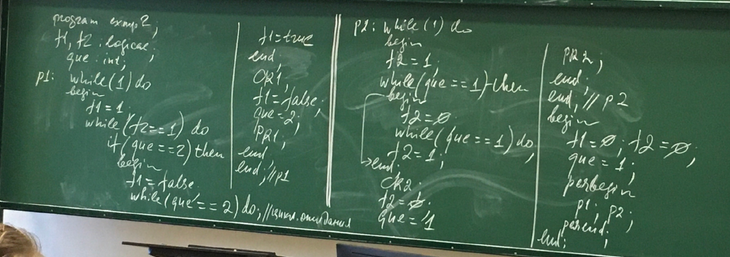
\includegraphics[width=\linewidth]{1}
	
	Засчет дополнительной переменной que (чья-очередь) получаем следующее. Процесс сразу захватывает свой флаг, затем проверяет флаг своего процесса. Если флаг другого процесса установлен, то выполняется проверка, чья очередь. Если очередь второго процесса, то флаг первого сбрасывается и переходит в цикл ожидания по переменной que. Выйдя из цикла ожидания, процесс устанавливает свой флаг, переходит в критический участок. Затем, сбрасывает первый флаг, отдает очередь другому процессу.
	
	\section*{Аппаратная реализация}
	
	В IBM370 появилась команда test-and-set. Эта команда является неделимой (атомарной) и реализует проверку и установку значения в памяти. Данная команда читает значение логической переменной b, копирует его в a, а затем для b устанавливает значение <<истина>>.
	
	Использование данной команды называется <<аппаратная реализация>> (у Вахалии - простой блокировкой).
	
	\begin{lstlisting}
program use_testandset;

fl, c1, c2: logical;

p1:
while(1) do
{
	c1 = 1;
	
	while(c1 == 1) do
		{testandset(c1, fl);}
	CR1;
	fl = 0;
	PR1;
}

p2:
while(1) do
{
	c2 = 1;
	
	while(c2 == 1) do
		{testandset(c2, fl);}
	
	CR2;
	fl = 0;
	PR2;
}

void main()
{
	fl = 0;
	
	parbegin
		p1; p2;
	parend;
}
	\end{lstlisting}

	Логическая переменная fl имеет значение <<истина>>, если один из процессов в CR.
	
	Пусть процесс P1 хочет войти в CR1, а P2 уже находится в CR2. P1 устанавливает переменную C1 = 1, затем входит в цикл проверки переменной fl командой test-and-set. Поскольку P2 в CR2, то fl = 1. Команда test-and-set обнаруживает это и устанавливает C1 = 1. В результате P1 находится в своем цикле активного ожидания до тех пор, пока P2 не выйдет из CR2 и не сбросит fl.
	
	Считается, что данный способ аппаратной реализации взаимоисключения не приведет к бесконечному откладываению (оно возможно, но его вероятность очень мала). Считается, что когда процесс выходит из своего CR и сбрасывает флаг, то, скорее всего, другой процесс сможет перехватить инициативу и переустановить флаг fl.
	
	Команда test-and-set активно используется в системах [что-то о циклической блокировке].
	
	Чаще всего команда test-and-set возвращает предыдущее значение какой-то логической переменной.
	
	[код spin\_lock]
	
	Реализация команды test-and-set во многих архитекутрах связана с блокировкой шины памяти. [...] может привести к занятию шины [...], что может привести к снижению отзывчивости системы. Решить эту проблему можно с помощью двух вложенных циклов.
	
	[код]
	
	Если переменная занята, то начинает выполняться обычный цикл проверки без захвата шины данных.
	
	\section*{Семафоры}
	
	В 1965 году Dijkstra E.W. опубликовал работу по взаимодействие параллельных процессов, в которой предложил семафоры как средство взаимоисключения. Семафор определяется следующим образом.
	
	Семафор - это неотрицательная защищенная переменная, на которой определены две неделимые операции, которые были названы P(S) и V(S).
	
	Операция P(S) уменьшает значение семафора на единицу. Декремент возможен, если S > 0. Если S = 0, то декремент невозможен и процесс блокируется до тех пор, пока декремент не станет возможным.
	
	V(S) - инкремент. В результате, процесс будет разблокирован.
	
	При этом к семафору может быть организована очередь. Когда семафор будет освобождден, то он захватит первый процесс в данной очереди.
	
	Если на семафоре определены два значения 0 и 1, то это бинарный семафор. Если целые положительные значения, то это считающий семафор.
	
	Если процесс не может захватить семафор, процесс блокируется (нет активного ожидания). Блокирован - не получает процессорного времени. Другой процесс, который освобождает семафор, то захват будет возможен. Однако семафор поддерживается ядром (все это работает в режиме ядра).
	
	[код]
	
	Яркий пример использования считающих семафоров - задача производства-потребления на трех семафорах (от Дейкстры):
	
	[собственно, сама задача]
	
	Доступна очередь и два типа процессов: производитель и потребитель. Производитель только записывает единицу данных, то есть заполнять ячейки буфера, а потребитель - только выбирать данные из буфера.
	
	Решение: использовать два считающих и один бинарный семафоры.
	
	Se - число пустых ячеек буфера;
	
	Sf - число запол.ненных ячеек буфера;
	
	Sb - бинарный семафор
	
	[код]
	
	{\bf Процессы явлются ассинхронными, и они выполняются с разной скоростью.} Предсказать, когда и какой процесс пройдет определенную точку, нельзя. Простое взаимоисключение не предусматривает синхронизацию.
	
	В современных системах реализованы наборы считающих семафоров (множественные семафоры). Возможности множественных семафоров рассмотрим на классической задаче <<Обедающие философы>>: на столе - пять тарелок, между которыми - по одному столовому прибору. Существует три способа действия философов:
	
	\begin{itemize}
		\item Каждый из философов пытается одновременно взять оба прибора;
		\item Каждый из философов пытается взять правый прибор и, удерживая его, пытается взять левую;
		\item Каждый из философов пытается взять правый прибор и, удерживая его, пытается взять левую. Если не удается, но правый прибор возвращается;
	\end{itemize}

	[код]
	
	\section*{Свойства наборов семафоров}
	
	\begin{itemize}
		\item Одной неделимой операцией может быть изменено значение всех или части наборов семафоров;
	\end{itemize}

	Почему появились наборы семафоров? [...]
\end{document}
